% !TeX root = ../../tesis.tex

% =============================================================================
\subsection*{Grupo 3: Topología y Rigor Matemático}
% =============================================================================

% -----------------------------------------------------------------------
\subsection{Centralidad de Intermediación (\termino{Betweenness Centrality}) \texorpdfstring{($B(v)$)}{(B(v))}}
\label{subsec:centralidad-intermediacion}
% -----------------------------------------------------------------------

\textbf{Fuentes principales:} \citet{lee2008}; \citet{allauca2023}

\subsubsection{Definición y Fundamentación}

La Centralidad de Intermediación ---denominada en la literatura anglosajona
\termino{betweenness centrality}--- cuantifica la importancia de cada nodo de la
red en función de cuántas rutas óptimas de la ciudad lo utilizan como nodo de
paso. Un nodo con alta centralidad de intermediación es aquel que aparece con
mayor frecuencia en los caminos mínimos entre los distintos pares origen-destino
del sistema: su remoción o saturación produce el mayor impacto sobre los tiempos
de viaje globales.

\citet{allauca2023} señala que la representación de la red de transporte como un
grafo permite realizar un análisis de centralidad para evaluar la importancia de
los nodos (estaciones), lo que sirve fundamentalmente para identificar los nodos
críticos y las rutas más importantes del sistema. \citet{lee2008}, en su caso de
estudio del metro de Seúl, aplican este principio empíricamente, demostrando que
en un sistema metropolitano la distribución del grado nodal sigue una ley de
potencias, confirmando la naturaleza de red libre de escala del sistema y su
consecuente vulnerabilidad a ataques dirigidos.

\subsubsection{Fórmula}

\begin{equation}
    B(v) = \sum_{s \neq v \neq t} \frac{\sigma_{st}(v)}{\sigma_{st}}
    \label{eq:betweenness}
\end{equation}

Donde:
\begin{itemize}
\item $B(v)$ = Centralidad de Intermediación de la estación $v$ (adimensional,
    normalizada en $[0, 1]$).
    \item $\sigma_{st}$ = Número total de caminos mínimos desde la estación de
    origen $s$ hasta el destino $t$.
    \item $\sigma_{st}(v)$ = Número de esos caminos mínimos que pasan
    forzosamente por la estación $v$.
\end{itemize}

La versión ponderada del indicador, $B(v, w)$, utiliza el tiempo de viaje real
como métrica de costo en la búsqueda de caminos mínimos, de modo que los nodos
contabilizados son aquellos que aparecen en las rutas más rápidas, no
necesariamente las más cortas en distancia.


\begin{figure}[H]
    \centering
    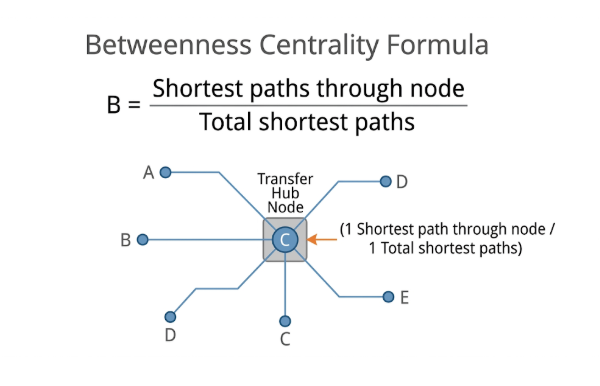
\includegraphics[width=0.62\textwidth]{Figures/Cap3/CentralidadItnermediacion.png}
    \caption[Diagrama de Centralidad de Intermediación $B(v)$]{Nodo de
    transferencia con alta centralidad: concentra el mayor número de caminos
    mínimos del sistema.}
    \label{fig:indicador-Bv}
    \fuentefigura{Elaboración propia con base en \citet{lee2008} y
    \citet{allauca2023}.}
\end{figure}


\subsubsection{Ejemplo Práctico: \cdmx{} y Zona Metropolitana}

\begin{table}[H]
    \centering
    \caption{Variación del indicador $B(v)$ antes y después del Anillo Periférico.}
    \label{tab:betweenness}
    \begin{tabularx}{\textwidth}{X r r r}
        \toprule
        \textbf{Nodo} & \textbf{$B(v)$ Red Actual} &
        \textbf{$B(v)$ con Anillo} & \textbf{Variación} \\
        \midrule
        Pantitlán               & $\approx 0.40$ & $\approx 0.22$ & $-45\%$ \\
        Pino Suárez             & $\approx 0.38$ & $\approx 0.20$ & $-47\%$ \\
        Tacubaya                & $\approx 0.35$ & $\approx 0.19$ & $-46\%$ \\
        Estaciones Anillo (prom.) & ---          & $\approx 0.18$ & $+\infty$ (nuevos) \\
        \bottomrule
    \end{tabularx}
\end{table}

La caída en la centralidad de intermediación de los nodos del centro de la
ciudad, combinada con el surgimiento de nuevos nodos de alta centralidad en el
Anillo Periférico, constituye la demostración algorítmica de que la propuesta
descongestiona el núcleo urbano y redistribuye los flujos hacia la periferia.

La implementación computacional de referencia para este indicador se encuentra
en el \autoref{anx:indicadores-implementacion} (§\ref{anx:impl-betweenness}).

La Centralidad de Intermediación es la métrica central del Objetivo Específico 3
(§\ref{subsec:obj-especificos}): identificar los nodos cuya pérdida
comprometería la conectividad global del sistema equivale a encontrar los nodos
que maximizan $B(v)$ en la red actual. Los valores de la tabla anterior
anticipan que Pantitlán, Pino Suárez y Tacubaya concentran desproporcionadamente
los flujos de la red radial, vulnerabilidad que el corredor anillar mitiga al
distribuir esa centralidad sobre nuevos nodos perimetrales.
